\subsection{Nature included in the game}


\begin{figure}[h]
\centering

  \centering
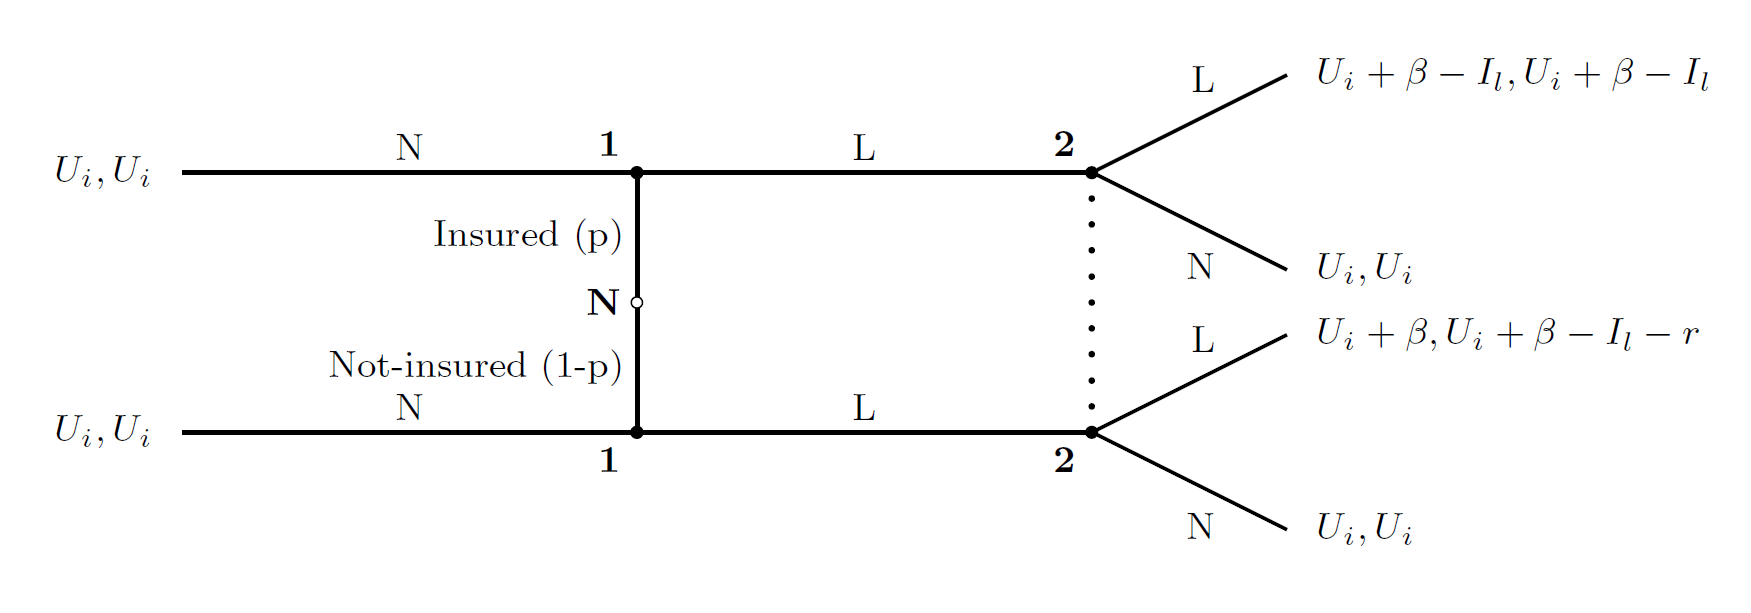
\includegraphics[width=1\linewidth]{../Figures/SignalingGameInsured.png}

\caption{TESTESTTEST}



\end{figure}
\begin{figure}[h]
\centering

  \centering
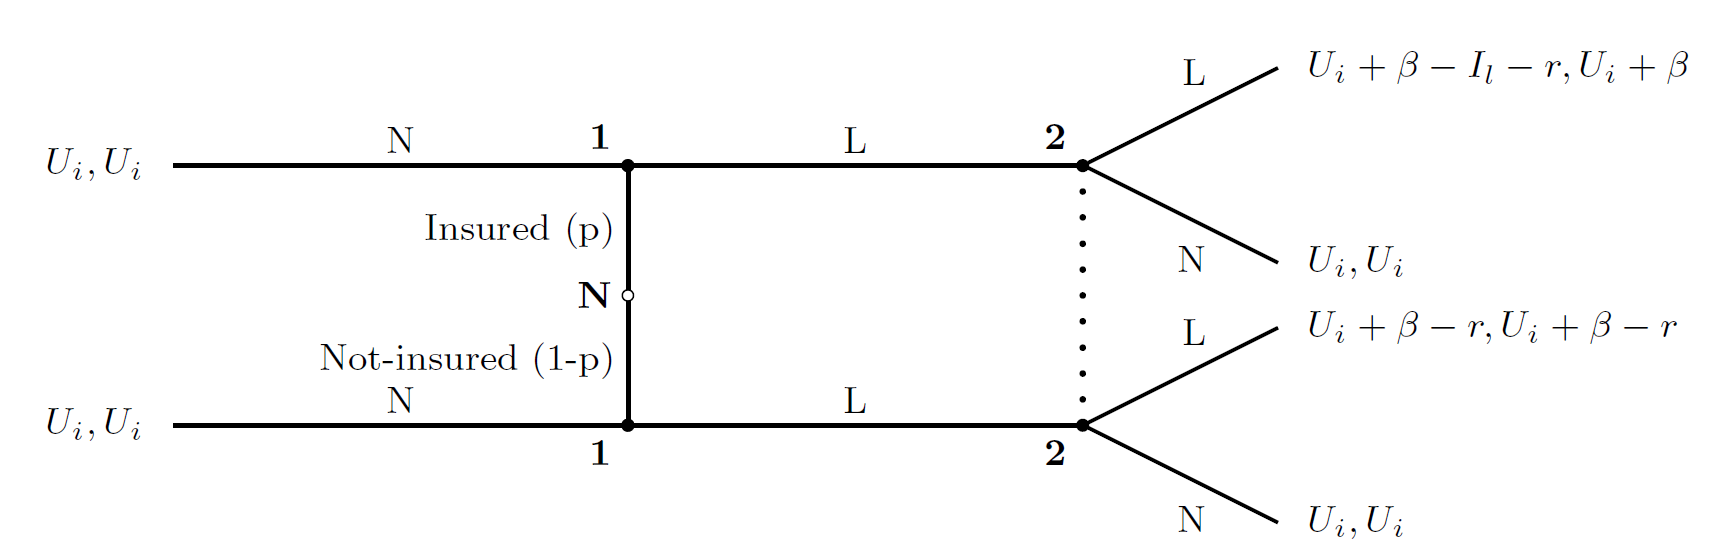
\includegraphics[width=1\linewidth]{../Figures/SignalingGameNotInsured.png}

\caption{TESTESTTEST}



\end{figure}

\subsection{Calculating the different equlibriums}
In this game we have two types of players, type 1$(t1)$: insured and type 2 $(t2)$: not insured. 
Player 1's type is chosen randomly by nature, with probability $p$ of being type 1 and $1-p$ of being type 2.
In this two person game player 1 have complete information, i.e. he knows his own and the other players type. Player 2 suffer has incomplete information and only knows his own type. 
In the extensiveform shown in figure \ref{fig:signalingInsured}, we see that $t2's$ strategy L dominates N, and thus $t2$ will never play $N$.
\subparagraph{Separating equilibrium}
If we can find a separating equilibrium, this will enable player 2 to distinguish the two possible types of player 1.
Since player 1 will never play $N$ as type 2, there are only one possible separating equlibrium, type 1 plays $L$ and type 2 plays $N$. Hence player 2's beliefs are as in equation \ref{eq:player2belief}.
\begin{equation}
    \sigma_{1}(t_{i})= 
\begin{cases}
   L,& \text{if } t1\\
   N,& \text{if } t2  
\end{cases}
\label{eq:player2belief}
\end{equation}
Let $\mu_{1}(t_{i} | N )$, denote the probability that player 1 is of type $t_{i}$. And by using bayes rule we get this equation:
\begin{equation}
\mu_{1}(t_{1} | N )=\frac{P(N|t_{1})P(t_{1})}{P(N)}=\frac{P(N|t_{1})P(t_{1})}{P(N|t_{1})P(t_{1})+P(N|t_{2})P(t_{2})}
\end{equation}
And with player 2's belief, we get that $\mu_{1}(t_{1} | N )=1$ and $\mu_{1}(t_{2} | L )= 1 $. Now we calculate player 2's expected utility from playing L and N:
\begin{eqnarray}
EU_{2}(L,L)=\mu_{1}(t_{1} | L )U_{2}(L,L;t_{1})+\mu_{1}(t_{2} | L )U_{2}(L,L;t_{2}) \nonumber\\
\llap{$\rightarrow$\hspace{50pt}}EU_{2}(L,L)=U_{i}+\beta-I_{l}-r \\
EU_{2}(N,L)=\mu_{1}(t_{1} | L )U_{2}(N,L;t_{1})+\mu_{1}(t_{2} | L )U_{2}(N,L;t_{2})\nonumber\\
\llap{$\rightarrow$\hspace{50pt}}EU_{2}(N,L)=U_{i}
\end{eqnarray}
From these two equations we see that the best response of player 2($BR_2$) when he observes the other player choosing action $L$ is:
\begin{equation}
BR_{2}(L)=
\begin{cases}
L, & \text{if }\beta - r \geq I_{l}\\
N, & \text{if } \beta -r<I_{l}
\end{cases}
\label{eq:insuredBR}
\end{equation}
Player 2's expected utility when type 1 chooses N, is easily seen to be $U_{i}$. 
To confirm if this is a separating equilibrium we must see if player 1 has any incentive to deviate from the strategies in player 2's belief.
Type 2 will never deviate, so lets investigate type 1.
For player 1 to be willing to play N when he knows player 2's best response function, this must hold: $\beta<I_{l}$. If this is true, then player 2's best response is to play N. I.e. the only separating equilibrium is the following:

\begin{eqnarray}
\beta<I_{l}\\
 \sigma_{1}= 
\begin{cases}
   L,& \text{if } t1\\
   N,& \text{if } t2  
\end{cases}\\
BR_{2}(\sigma_{1})=N
\end{eqnarray} 
\subparagraph{Pooling equilibrium}
In a pooling equilibrium player 2 will not be able to distinguish the two types, and since $t1$'s strategy $L$ dominates $N$, i.e. there is only one possible equilibrium, the one where both types of player 1 plays $L$.
\begin{equation}
    \sigma_{1}(t_{i})= 
\begin{cases}
   L,& \text{if } t1\\
   L,& \text{if } t2  
\end{cases}
\label{eq:player2beliefpooling}
\end{equation}
By using bayes rule we get that $\mu(t_{1}|L)=p$ and $\mu(t_{2}|L)=1-p$.
Player 2's expected utility is then:
\begin{eqnarray}
EU_{2}(L,L)=p(U_{i}+\beta-I_{l})+(1-p)(U_{i}+\beta-I_{l}-r)\nonumber\\
\llap{$\rightarrow$\hspace{50pt}}EU_{2}(L,L)=U_{i}+\beta-I_{l}-r+r\\
EU_{2}(N,L)=U_{i}
\end{eqnarray}
From this we get player2's best response:
\begin{equation}
BR_{2}(L)=
\begin{cases}
L ,& \text{if } \beta + rp-r\geq I_{l} \\
N ,& \text{if } \beta +rp -r < I_{l} 
\end{cases}
\end{equation}
By using this best response function, player 1 sees that as long as $\beta>I_{l}$ he will never deviate from player 2's beliefs. And it is a pooling equilibrium where both player choose $L$, as long as $\beta>I_{l}$ and $\beta +rp-r>I_{l}$.
If $\beta>I_{l}$ but $\beta +rp-r<I_{l}$, we have a pooling equilibrium where player 1 plays $L$, and player 2 plays $N$. 
\begin{figure}[h]
\centering

  \centering
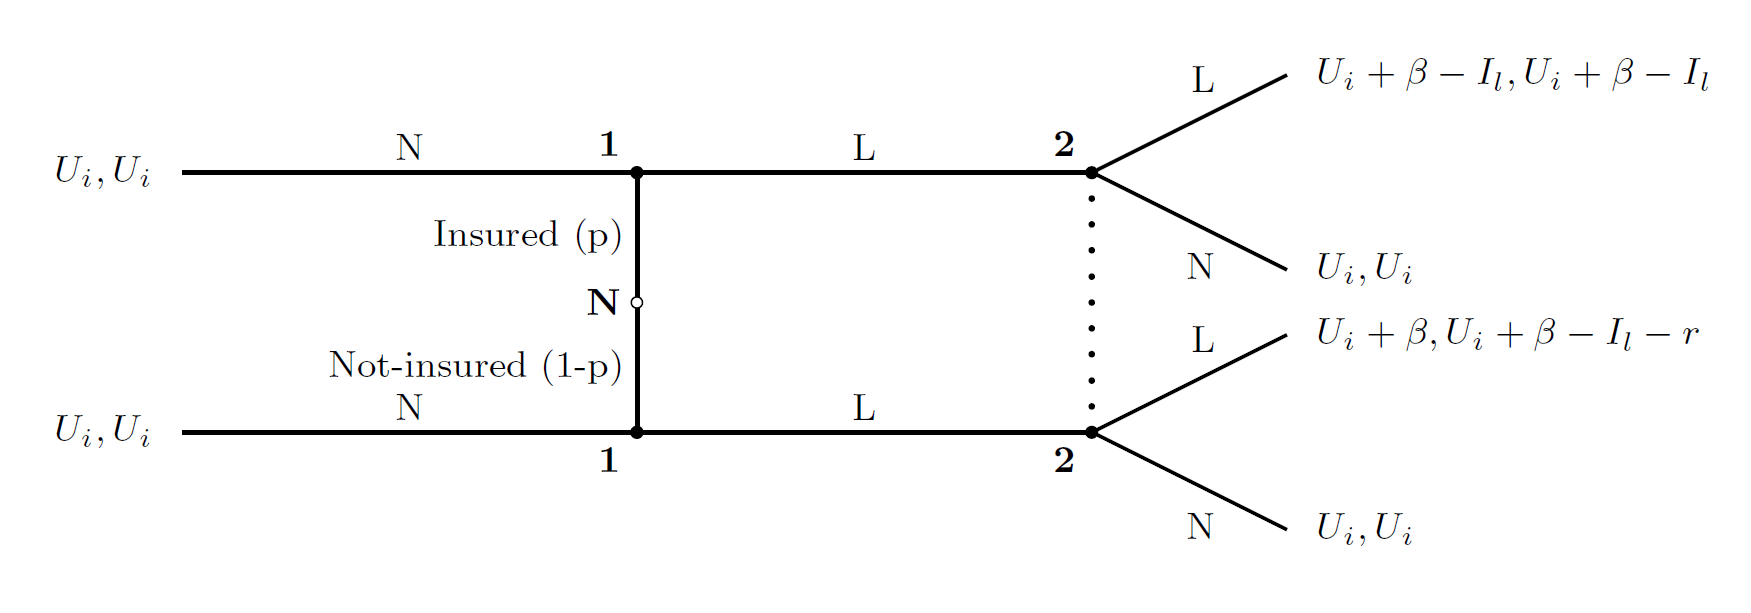
\includegraphics[width=1\linewidth]{../Figures/SignalingGameInsured.png}

\caption{Appendix XXXX signaling game with nature \label{fig:signalingInsured}}



\end{figure}